
\chapter{Method 2: Tri-dexel}
\label{ch:tri_dexel}

The second discussed method to extract a triangulated surface from the VML's data model is based on a tri-dexel representation, \cf section \ref{sec:surface_representations}.
As observed with the previously shown method in chapter \ref{ch:direct_intersection}, reconstructing a surface directly form the many intersecting triangles stored in the VML's grid is computationally expensive, highly numerically unstable and prone to errors.
A more robust approach is desirable, which is able to always successfully reconstruct a surface with good quality.
This reconstruction should succeed independently of the complexity of the maintained geometry.
As a trade-off for this robustness, the approach may sacrifice surface exactness and filigree features.
Dexel-based representations fit this purpose nicely.
They provide a good abstraction of a machined workpiece with rich semantics.
The used grid resolution supplies an easy to configure level of detail and steering parameter between representation quality and memory/CPU demands.
Creating dexel-based representations from the VML's data model is achieved using an adaption of the already implemented and well-working raycasting subsystem used for visualization, \cf section \ref{sec:raycasting}.
To achieve a good portrayal independently of the workpiece's orientation, three axis-aligned dexel images will be generated, thus creating a tri-dexel representation.
For converting such a tri-dexel model into a final triangle mesh, various algorithms are found in literature.
An excellent example is Ren \etal's "Feature Conservation and Conversion of Tri-dexel Volumetric Models to Polyhedral Surface Models for Product Prototyping" \cite{tridexel_reconstruction}.
Their approach form the idea and foundation of the implementation presented in this chapter.


\section{Concept}
\label{sec:tri_dexel_concept}


\begin{figure}
	\centering
	\begin{subfigure}[t]{0.3\textwidth}
		\centering
		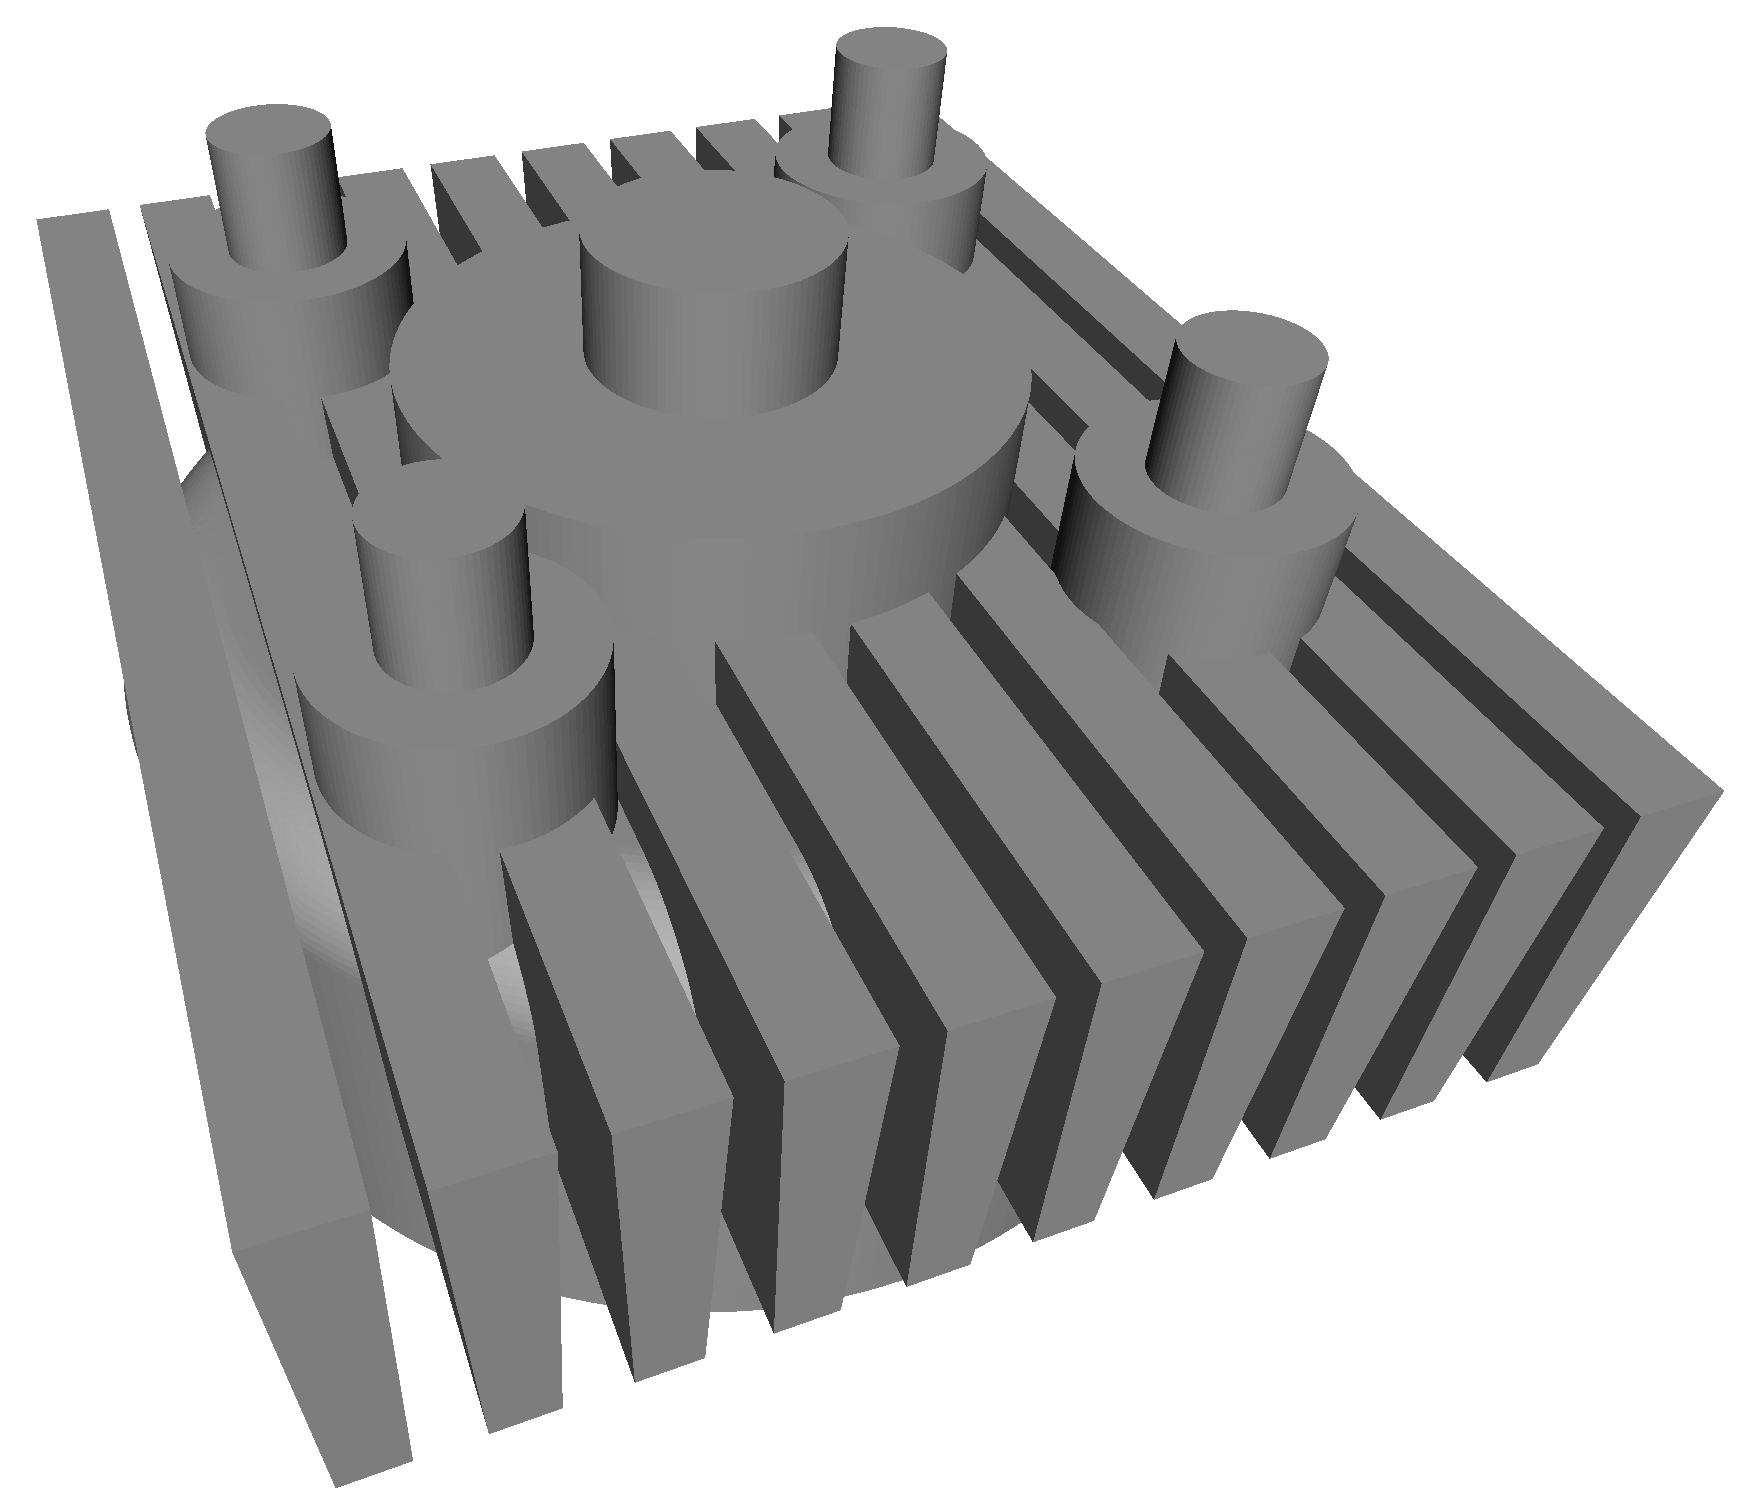
\includegraphics[width=\textwidth]{images/cylinder_head_stock_and_svs}
		\caption{Stock and SVs}
		\label{fig:cylinder_head_stock_sv}
	\end{subfigure}
	\begin{subfigure}[t]{0.3\textwidth}
		\centering
		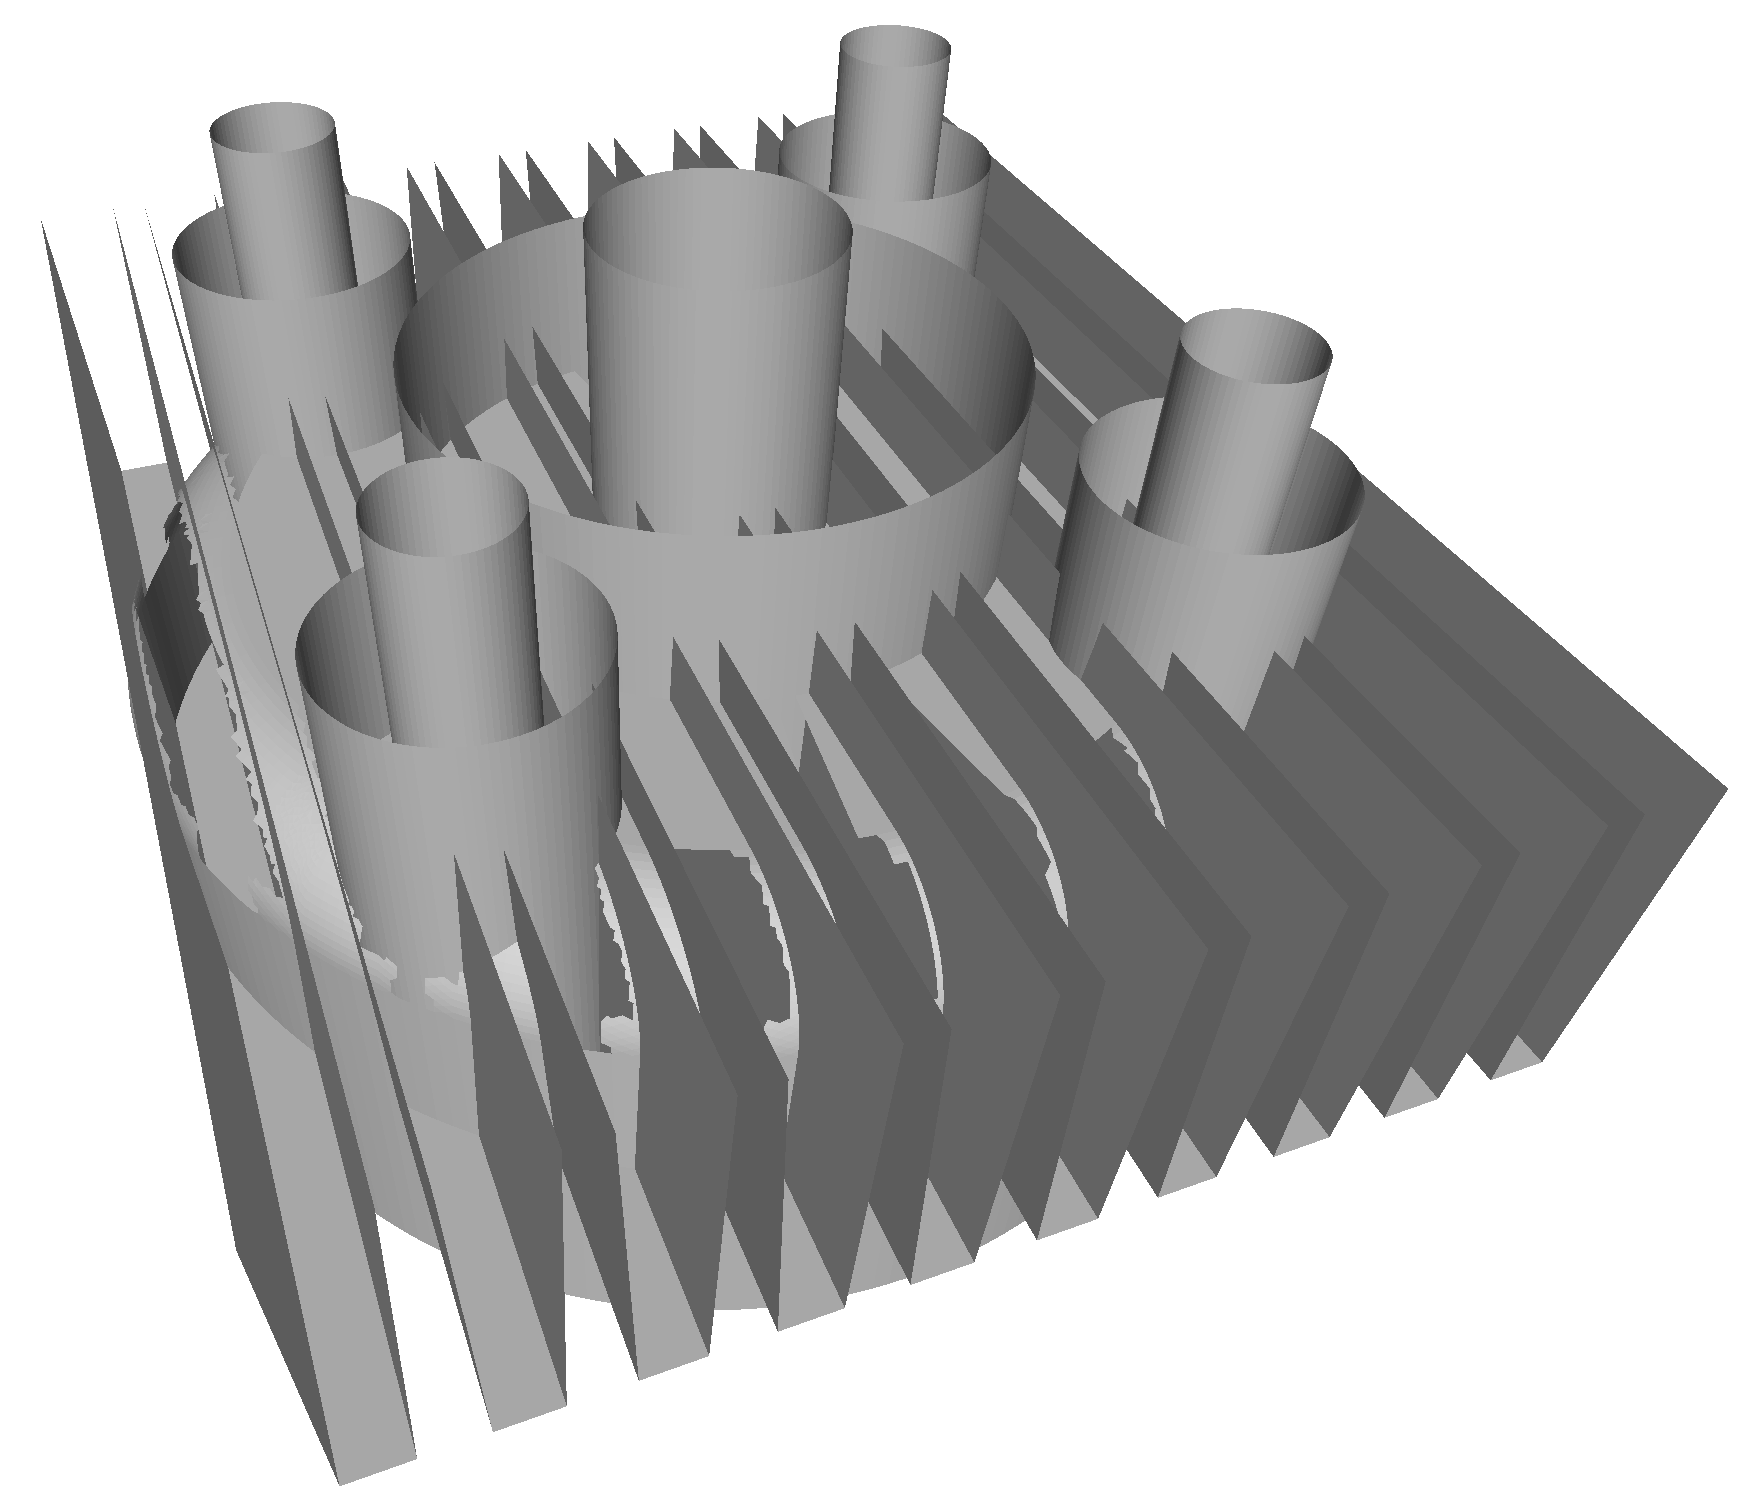
\includegraphics[width=\textwidth]{images/cylinder_head_vml}
		\caption{VML}
		\label{fig:cylinder_head_classified}
	\end{subfigure}
	\begin{subfigure}[t]{0.3\textwidth}
		\centering
		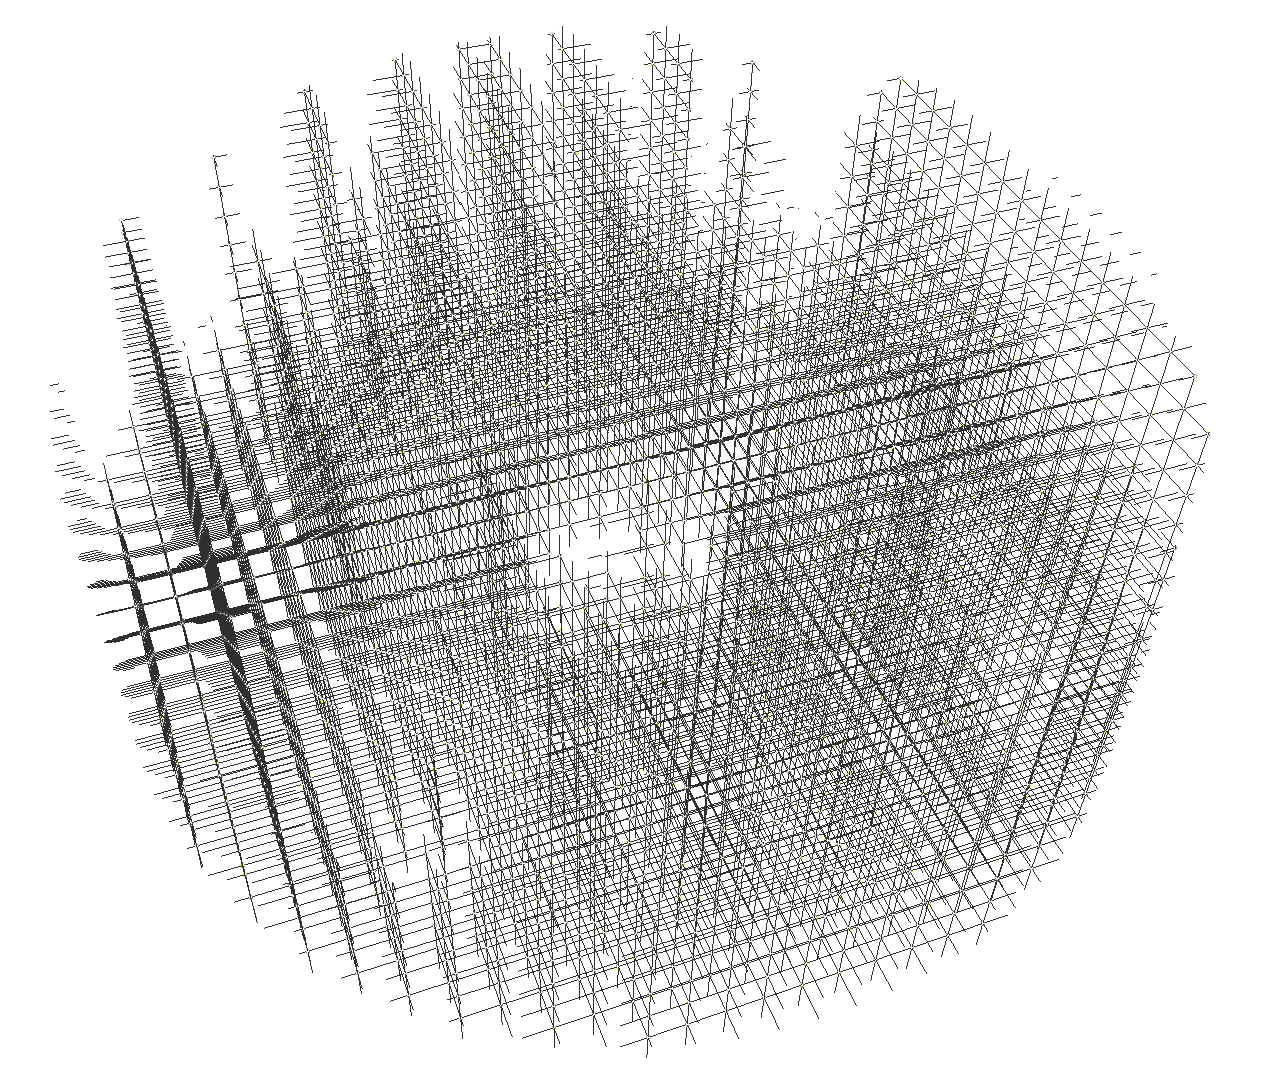
\includegraphics[width=\textwidth]{images/cylinder_head_dexel_image}
		\caption{Tri-dexel image}
		\label{fig:cylinder_head_dexel_image}
	\end{subfigure}
	\begin{subfigure}[t]{0.3\textwidth}
		\centering
		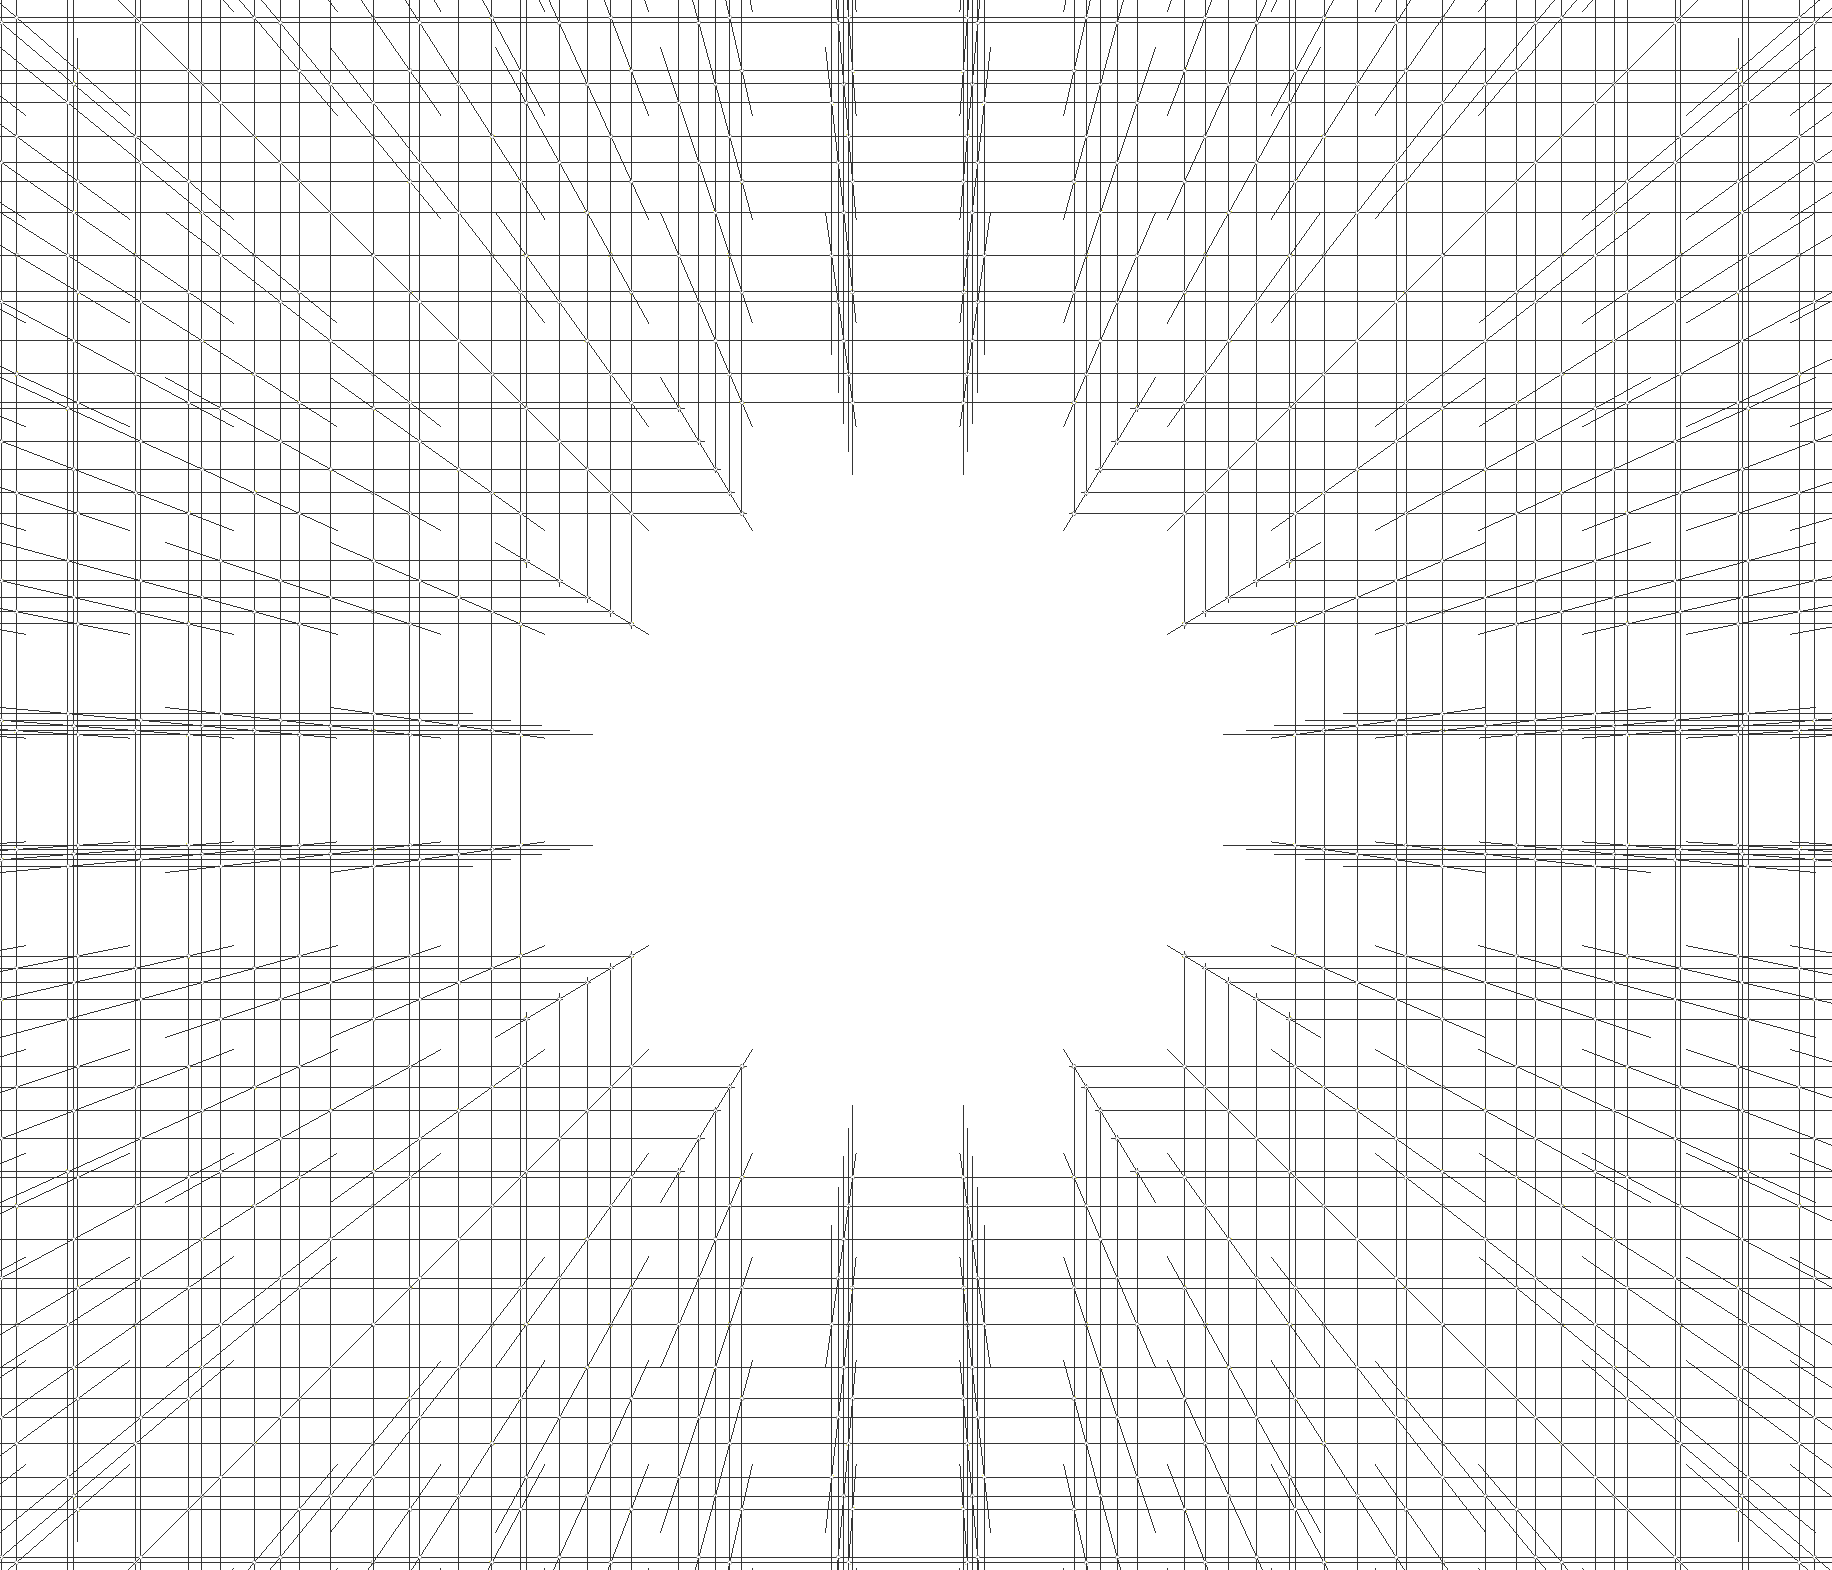
\includegraphics[width=\textwidth]{images/cylinder_head_dexel_image_center}
		\caption{Tri-dexel image center}
		\label{fig:cylinder_head_dexel_image_center}
	\end{subfigure}
	\begin{subfigure}[t]{0.3\textwidth}
		\centering
		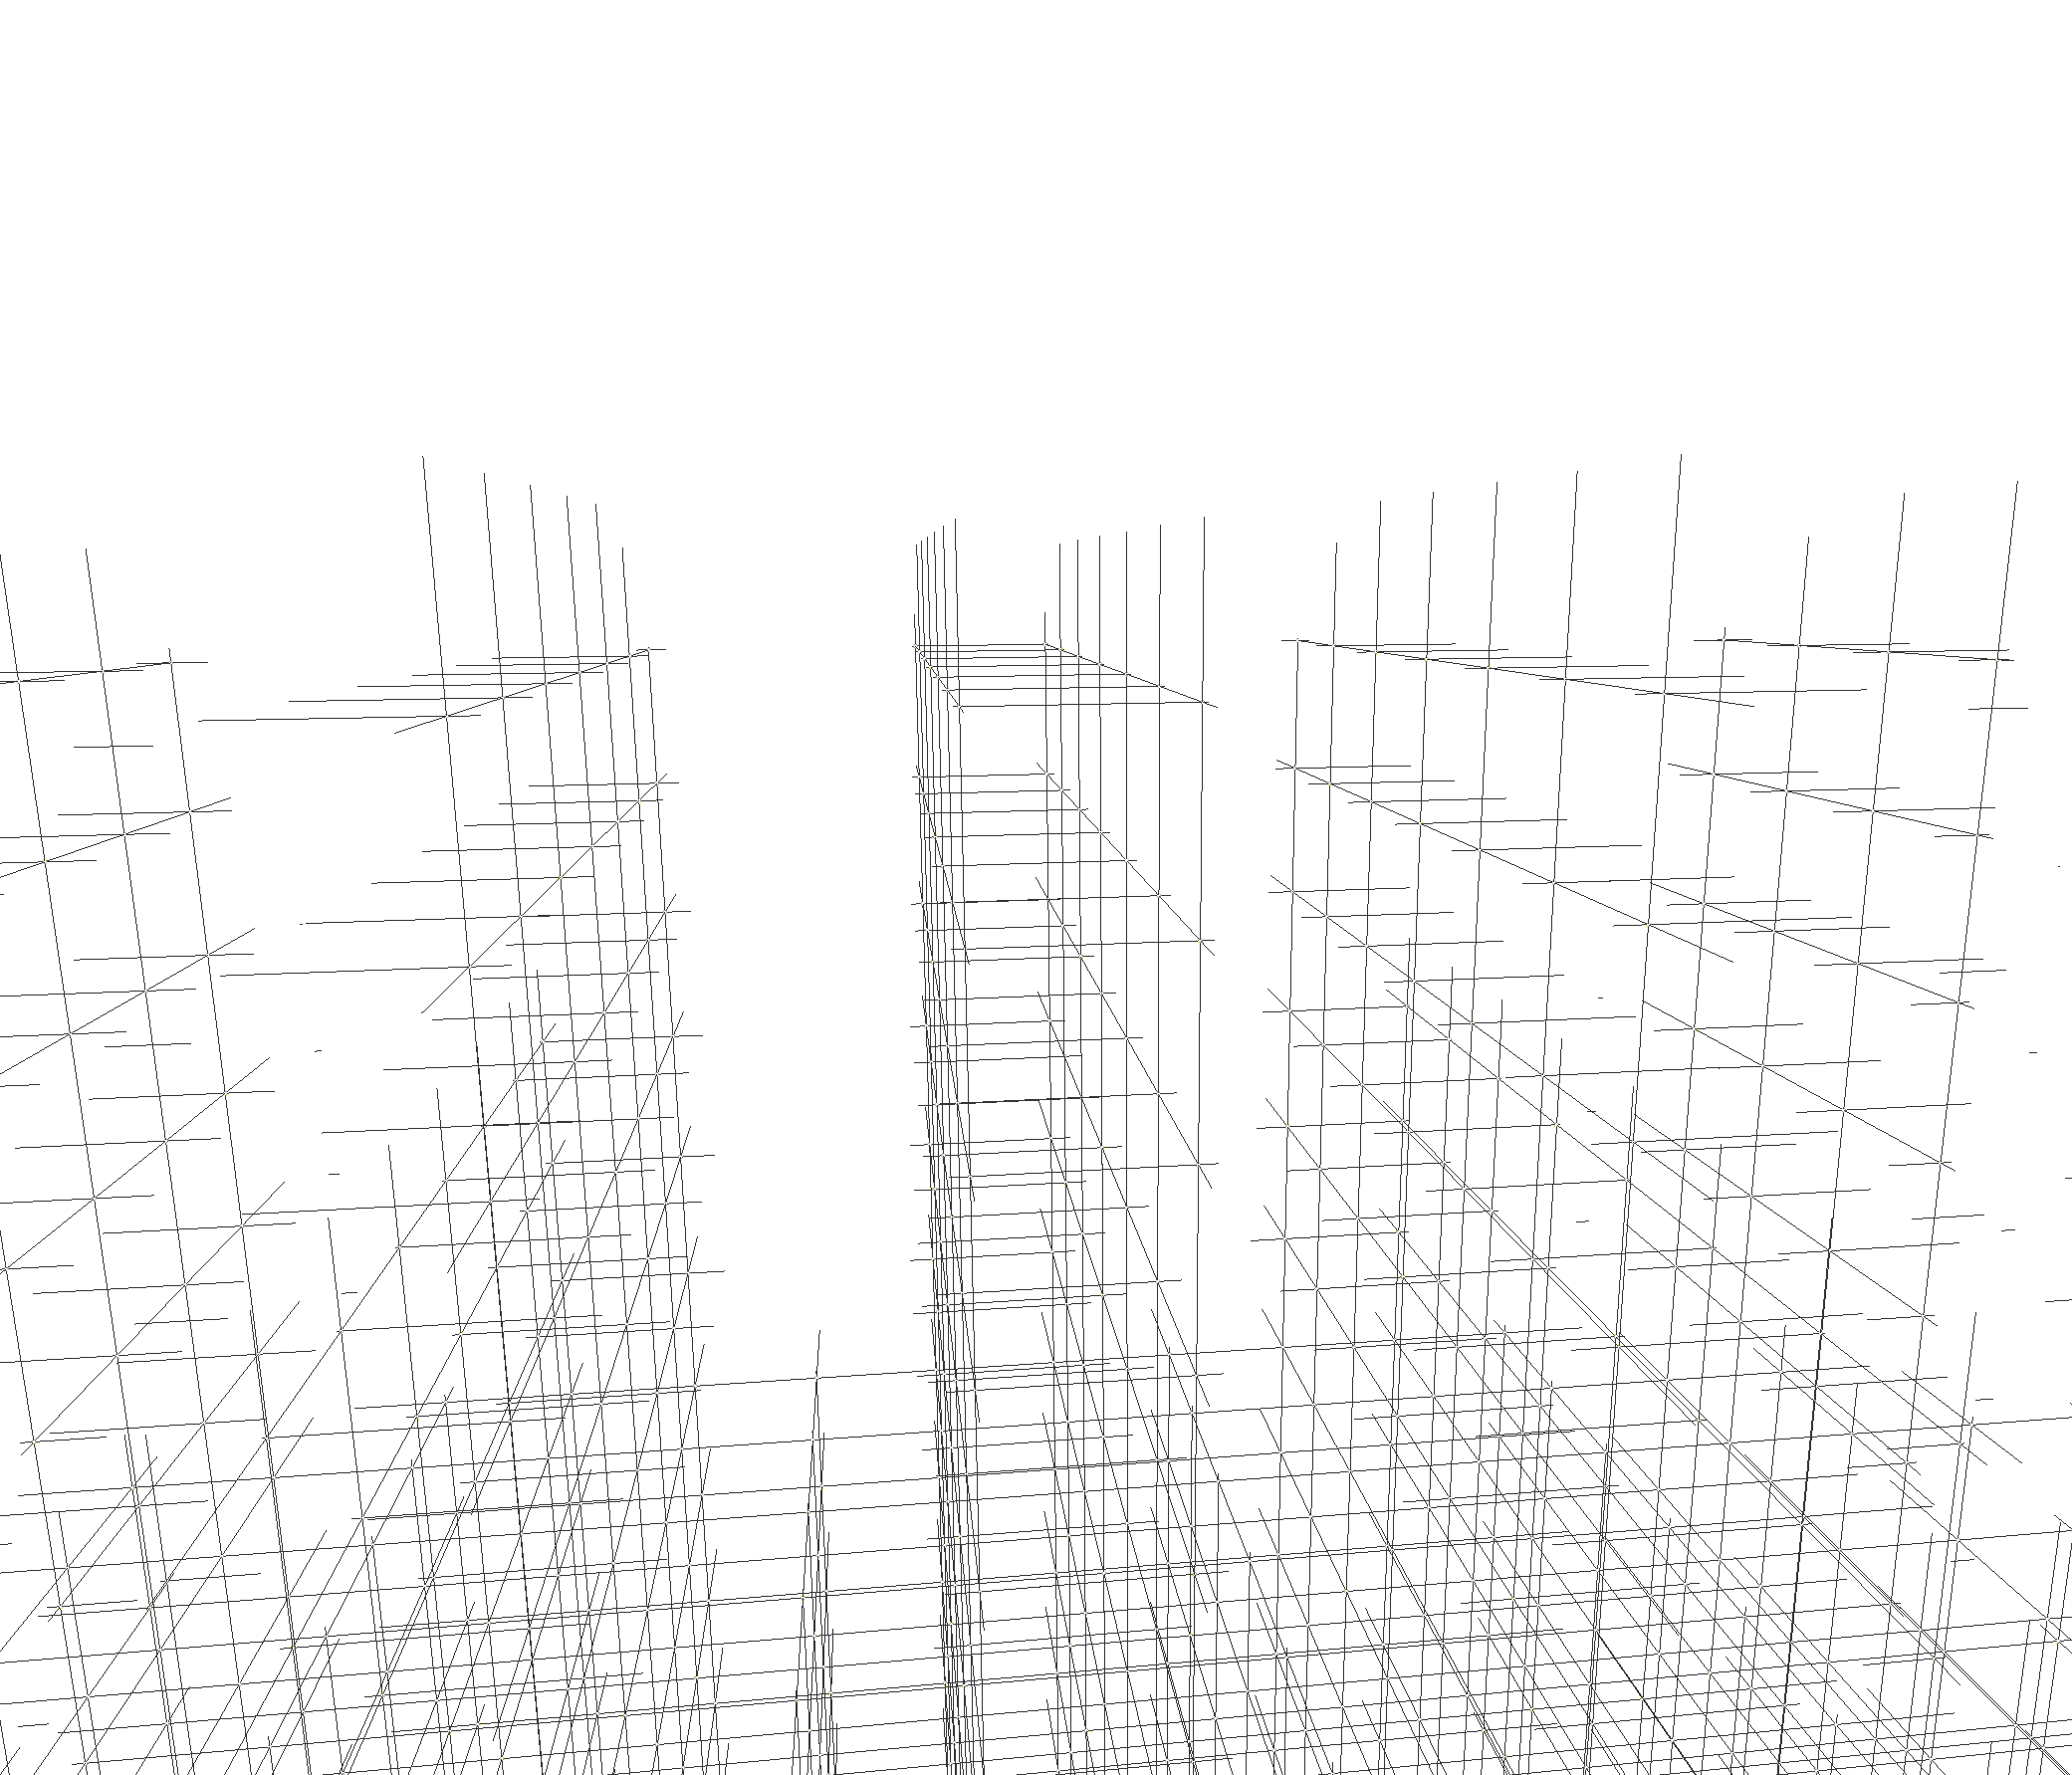
\includegraphics[width=\textwidth]{images/cylinder_head_dexel_image_fins}
		\caption{Tri-dexel image fins}
		\label{fig:cylinder_head_dexel_image_fins}
	\end{subfigure}
	\begin{subfigure}[t]{0.3\textwidth}
		\centering
		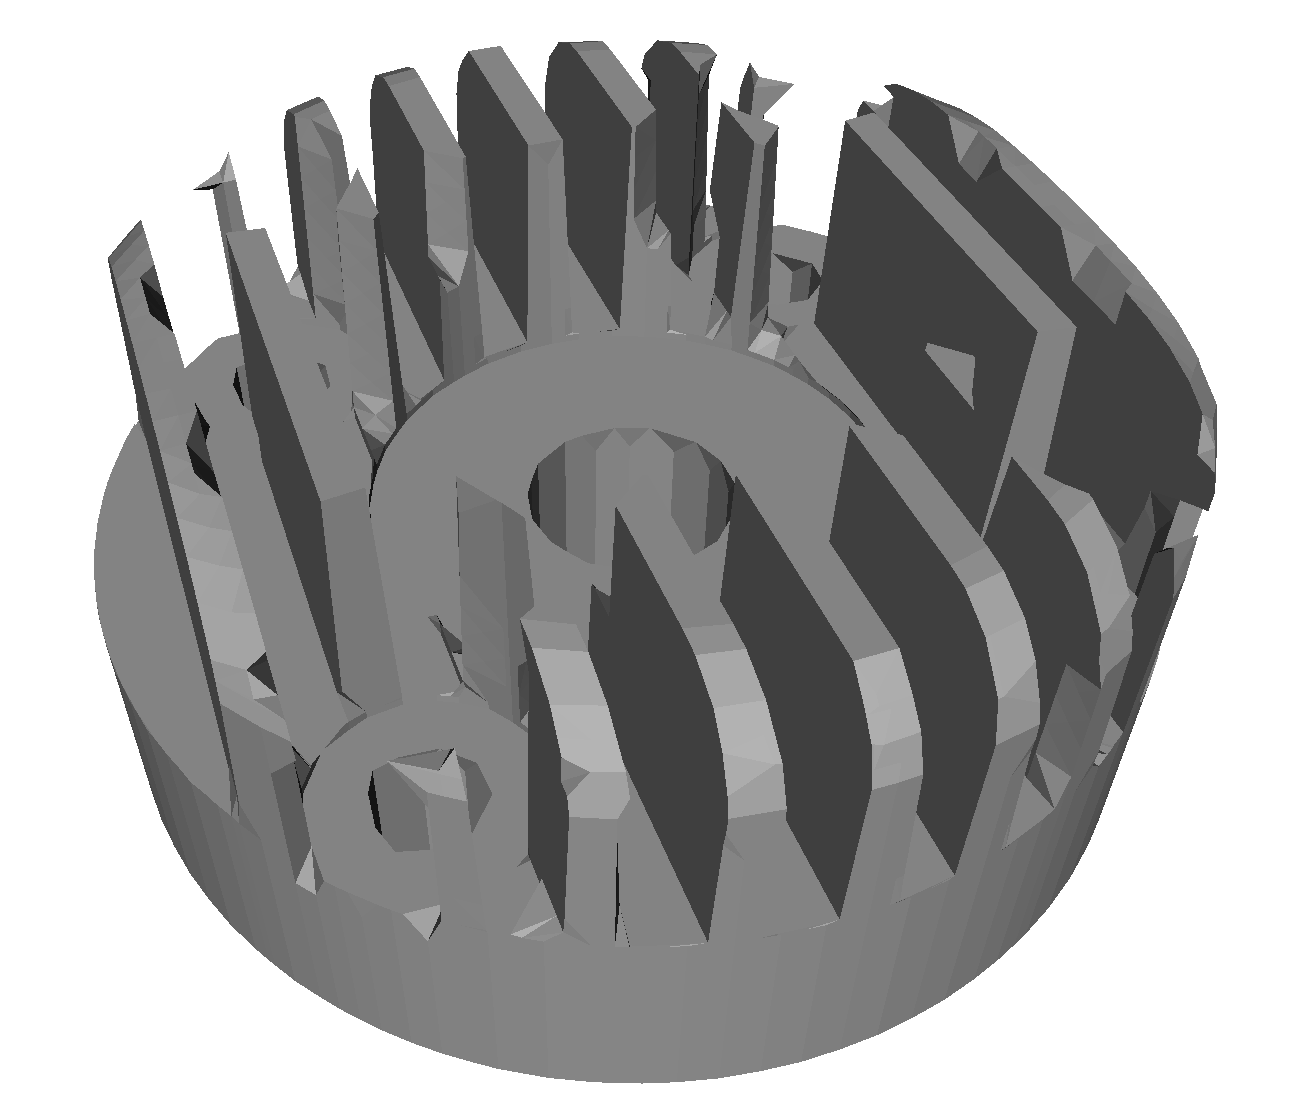
\includegraphics[width=\textwidth]{images/cylinder_head_reconstructed}
		\caption{Result}
		\label{fig:cylinder_head_reconstructed}
	\end{subfigure}
	\caption{
		Tri-dexel based surface reconstruction from the VML's data model of a cylinder head.
		Figure \ref{fig:cylinder_head_stock_sv} shows the stock and a few swept volumes creating the fins and drillings.
		Figure \ref{fig:cylinder_head_classified} shows the classification result after these solids have been mapped into the VML's regular grid.
		The removed triangles are clearly visible, especially at the swept volumes.
		By using a raycast of axis parallel rays along all three coordinate system axes a tri-dexel representation is created as shown in figure \ref{fig:cylinder_head_dexel_image}.
		The resolution of the grid spawning the rays is 30 along the longest dimension.
		Figure \ref{fig:cylinder_head_dexel_image_center} and \ref{fig:cylinder_head_dexel_image_fins} show details of the tri-dexel image.
		The former views the drilling at the center from above and the latter views the cylinder head's fins from the center.
		Finally, the reconstructed surface is shown in figure \ref{fig:cylinder_head_reconstructed}.
		Note the imperfections at the fin's edges and bases.
	}
	\label{fig:cube2}
\end{figure}


\section{Implementation}
\label{sec:tri_dexel_implementation}



\subsection{Raycast}
\label{sec:tri_dexel_raycast}



\subsection{Dexel image generation}
\label{sec:tri_dexel_dexel_image_generation}



\subsection{Regularization}
\label{sec:tri_dexel_regularization}



\subsection{Triangulation}
\label{sec:tri_dexel_triangulation}



\subsection{Refinement and feature reconstruction}
\label{sec:tri_dexel_refinement}



\subsection{Subslicing *experimential*}
\label{sec:tri_dexel_subslicing}



\subsection{Parallelization}
\label{sec:tri_dexel_parallelization}



\section{Results}
\label{sec:tri_dexel_results}


